\documentclass[letterpaper, 12pt]{article}
\usepackage[margin=1in]{geometry}
\usepackage{multicol}
\usepackage{graphicx}
\graphicspath{{Figures/}{./}}
\usepackage{apacite}
\usepackage{amsmath}
\usepackage{amssymb}
\usepackage{amsthm}
\usepackage{indentfirst}
\usepackage[justification=centering]{caption}
\usepackage{float}
\usepackage{tabularray}
\usepackage{listings}
\usepackage{url}
\lstset{
    breaklines=true,                    % sets automatic line breaking
%   breakatwhitespace=false,            % sets if automatic breaks should only happen at whitespace
    prebreak = \raisebox{0ex}[0ex][0ex]{\ensuremath{\hookleftarrow}} % just as an example
}


\usepackage{color}
\definecolor{lightgray}{rgb}{.9,.9,.9}
\definecolor{darkgray}{rgb}{.4,.4,.4}
\definecolor{purple}{rgb}{0.65, 0.12, 0.82}
\lstdefinelanguage{JavaScript}{
    keywords={break, case, catch, continue, debugger, default, delete, do, else, finally, for, function, if, in, instanceof, new, return, switch, this, throw, try, typeof, var, void, while, with},
    morecomment=[l]{//},
    morecomment=[s]{/*}{*/},
    morestring=[b]',
    morestring=[b]",
    sensitive=true
}
\lstset{basicstyle=\footnotesize,breaklines=true}
\pagenumbering{roman}

\title{MATHEMATICS ANALYSIS AND APPROACHES HL
\\
Producing the IB Logo with the Fourier Series}
\author{}
\date{}

\begin{document}
\nocite{*}

\maketitle
\begin{center}
    Candidate Code:
    \\
    Session: May 2024
    \\
    Page Count:
\end{center}
\newpage

\tableofcontents
\newpage


\pagenumbering{arabic}
\setcounter{page}{1}

\section{Introduction and Rationale}

I have shown interest in visual arts done through the means of software,
with particular experience in 3D modelling and animation in Blender
and Cinema 4D. It was the ability for the software to interpret
any decision the artist makes with accuracy, and there is without
a doubt that the software is composed of numerous moving parts.
Another related type of digital art is vector art in ".svg" files, which
in its own already relate
to mathematics in the sense that it contains numerous graphed mathematical
relationships in order to produce an image.

It was until I discovered an application of Fourier Series,
a summation of sinusoidal functions, that involved converting
these vector art pieces into a single series.
I found this to be incredibly intriguing, as it
requires just one expression to produce the same result done by the numerous mathematical
relationships. It is comparable to what are known as "one-liners"
in the programming community, where some take it as a challenge to
solve a programming problem that has a trivial multistep solution
into just one line of code. I've always been admired by those
who are able to come up with these concise solutions, and I
perceive the idea of representing an ".svg" file as a Fourier Series
to be a "one-liner" version in the area of math.

Traditionally, the Fourier Series is in the form of a summation
of cosine and sin functions, which in the context of this investigation
would necessitate finding two separate Fourier Series for the
x and y plane. However, there is also a form of the Fourier Series
represented as a summation of \(e^{it}\) terms. This
form is more preferable in this investigation, as not only
will this form allow for a single Fourier Series accounting
for both a horizontal and vertical axis but also extend
the breadth of this investigation into the realm of
complex numbers.


\section{Aim and Methodology}

The objective of this investigation is to link Fourier series with
complex numbers to create a single series that is capable
of reproducing the IB logo on the Argand plane.

The common sine-cosine form of the Fourier Series
involves calculus, series, and trigonometry.
To lay the foundations surrounding Fourier Series,
an example will be explored in Section \ref*{sec:overarchingIdea}
that will demonstrate the overarching idea of a Fourier Series
for a simple periodic function as well as how
the Fourier Series would be evaluated.

The area of complex numbers will then be introduced, where
after connecting the relevance of Euler's formula
to Fourier Series, an understanding of the mechanism of the Fourier Series
using complex numbers will be developed.

Next, Bezier Curves will be explored, which involves
polynomials to control the "lerp" of the Bezier Curve and
complex numbers to define a 2 dimensional position on the Argand
Plane. It will then become evident that the necessity
for Bezier Curves comes from its ubiquitous presence
in the ".svg" file of the IB logo.

Finally, the render of the IB logo will be
done with the aid of computer programming, which is essential in
this investigation involving the computation of the numerous integrals evaluated as Riemann Sums,
the computation of the extensive Fourier Series
as well as presenting the resulting graph on the Argand plane
through plotted pixels in an image. For this investigation,
a JavaScript program will be written with NodeJS as the runtime \cite{NodeJs}.
JavaScript NPM packages will offer additional preprogrammed tools,
with the following packages used in this investigation:

\begin{itemize}
    \item "mathjs" \cite{dejongMathjs}: Allows computation with complex numbers
    \item "read-excel-file" \cite{kuchumovReadexcelfile}: Allows reading the Excel spreadsheet containing data of the original IB logo
    \item "canvas" \cite{automatticCanvas}: Allows the result to be rendered on an image
    \item "prompt-sync" \cite{fragomeniPromptsync}: Enables input during the program's runtime through a command line interface
\end{itemize}

% \section{Plan of Action}

% This exploration focuses on the following areas of math:
% \begin{itemize}
%     \item Integral Calculus
%     \item Series
%     \item Trigonometry
%     \item Complex Numbers
%     \item Vectors
% \end{itemize}

\section{Background Information}

\subsection{Overarching idea of the Fourier Series} \label{sec:overarchingIdea}

A periodic function is one where the output for a particular input equals to
the output for the sum of the same input and the value of the function's period.
This can be represented mathematically as:
\begin{align*}
     & f(x) = f(x + P)
    \\
     & \text{where } P = \text{ the period of the function}
\end{align*}

The sine wave is widely known for being a periodic function for the ease of graphing
a sinusoidal wave. However, there are periodic functions that are difficult to
graph with an algebraic expression, such as one that alternates between
1 and -1 or one that is shaped as a zigzag.

This is the motivation behind the Fourier Series, which is to be able to represent
period functions that normally can't be represented by an algebraic function.

The idea behind the Fourier Series is to take an infinite sum of varying sinusoidal
functions such that a desired periodic function is produced.

\begin{figure}[H]
    \centering
    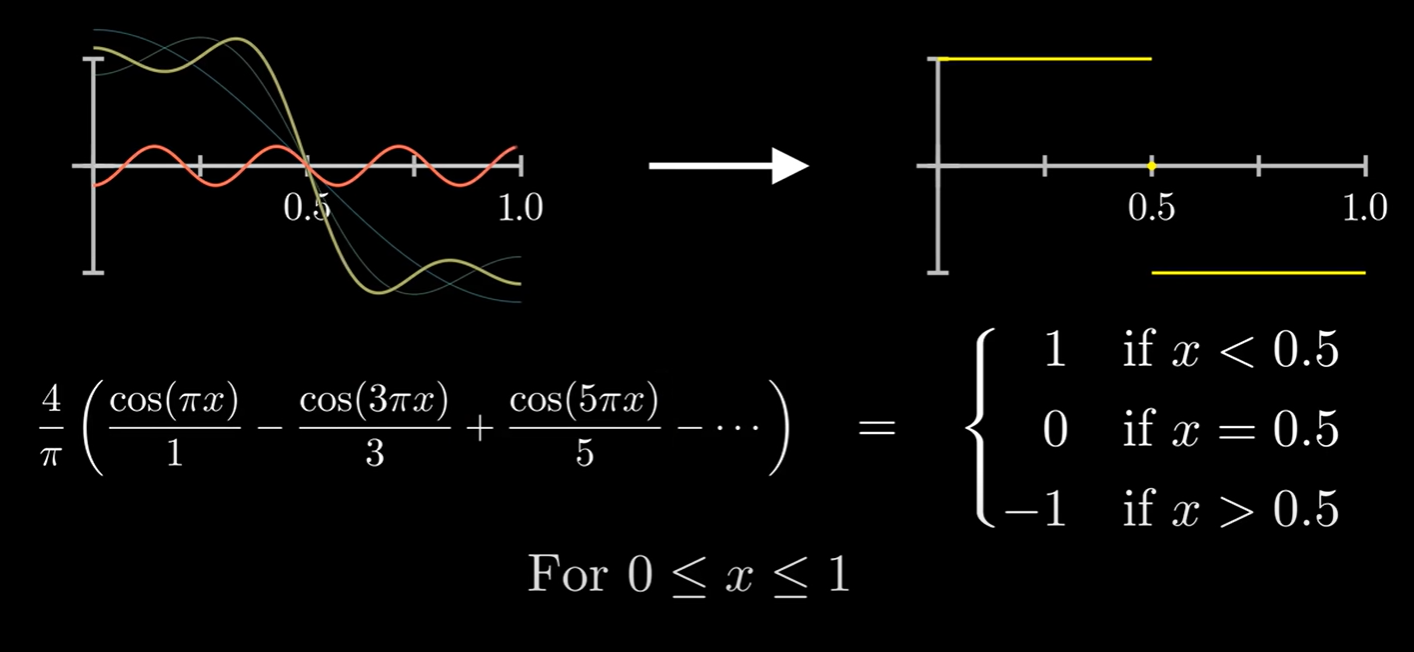
\includegraphics[width=\textwidth]{fourier_basic_visual.png}
    \caption{Visualization of the mechanism of the Fourier Series \protect\cite{sandersonWhatFourierSeries2019}. The purple line is the periodic function resulting from the previous iteration, the blue line is the sinusoidal function to be added in the next iteration.}
    \label{fig:fourier_visual}
\end{figure}
% (\( \frac{4}{\pi} \left( \frac{} \right) \))

The form of the Fourier Series in Equation \ref*{eq:sincos_form} is considered
to be the sin-cosine form and was the formula used to determine
the Fourier Series of the function in Figure \ref*{fig:fourier_visual}.
This is the most common form of the Fourier Series
as it is capable of modelling periodic functions such as
sawtooth waves and square waves that can't be expressed
in any other way yet are common in the real world \cite{FourierSeriesDefinition}.
It is also crucial in solving partial differential equations
such as the heat equation \cite{sandersonWhatFourierSeries2019}.

\begin{equation}
    \label{eq:sincos_form}
    f(t) = a_0 + \sum_{n=1}^{\infty} (a_n \cos \frac{n\pi x}{L} + b_n \sin \frac{n\pi x}{L})
\end{equation}

\[
    \text{Where } L = \text{Half of the period of the function}
\]

\begin{equation}
    \label{eq:a_not}
    a_0 = \frac{1}{2L} \int_{-L}^{L} f(x) \,dx
\end{equation}
\begin{equation}
    \label{eq:a_n}
    a_n = \frac{1}{L} \int_{-L}^{L} f(x) \cos \frac{n\pi x}{L} \,dx
\end{equation}
\begin{equation}
    \label{eq:b_n}
    b_n = \frac{1}{L} \int_{-L}^{L} f(x) \sin \frac{n\pi x}{L} \,dx
\end{equation}

Note: Equations \ref*{eq:sincos_form} to \ref*{eq:b_n} came from \cite{tisdellHowComputeFourier2009}.

For calculations of a Fourier Series using the sine-cosine form,
it is important to consider whether the function of concern
is even or odd. This is because integrating an odd function
from \(-L\) to \(L\) would always equal to zero,
with the mathematical explanation shown below.

\begin{align*}
     & I_{odd} = \int_{-L}^{L} f(x) \,dx = \int_{-L}^{0} f(x) \,dx + \int_{0}^{L} f(x) \,dx
    \\
     & \int_{-L}^{0} f(x) \,dx = -\int_{0}^{L} f(x) \,dx
    \\
     & \therefore I_{odd} = 0
\end{align*}

Additionally, any integral of an even function from \(-L\) to \(L\) can be simplified
as shown below.

\begin{align*}
     & I_{even} = \int_{-L}^{L} f(x) \,dx = \int_{-L}^{0} f(x) \,dx + \int_{0}^{L} f(x) \,dx
    \\
     & \int_{-L}^{0} f(x) \,dx = \int_{0}^{L} f(x) \,dx
    \\
     & \therefore I_{even} = 2\int_{0}^{L} f(x) \,dx
\end{align*}

Finally, while \(a_n\) and \(b_n\) both involve multiplying
two even/odd functions together, there is a method of
predicting the type of function that will result.

\begin{itemize}
    \item Multiplying even by even produces even because the two same signs of \(y\) will emerge for \(x < 0\) and \(x > 0\)
    \item Multiplying even by odd produces odd because the signage of \(y\) for one of \(x < 0\) or \(x > 0\) must be positive and the other negative
    \item Multiplying odd by odd produces even because either the signage of \(y\) in the two functions will be opposite for both \(x < 0\) and \(x > 0\) or the signage will be equal, therefore producing a final signage for \(y\) of negative and positive respectively.
\end{itemize}

The determination of the Fourier Series of the function in Figure \ref*{fig:fourier_visual}
is therefore shown below.

\begingroup
\allowdisplaybreaks
\begin{align*}
     & f(x) = \begin{cases}
                     & \vdots          \\
                  -1 & -1.5 < x < -0.5 \\
                  1  & -0.5 < x < 0.5  \\
                  -1 & 0.5 < x < 1.5   \\
                     & \vdots
              \end{cases}
    \\
     & f(x) = f(x + 2)
    \\
     & \therefore 2 = 2L
    \\
     & L = 1
    \\
    \\
     & a_0 = \frac{1}{2L} \int_{-L}^{L} \underbrace{f(x)}_{even} \,dx
    \\
     & = \frac{1}{2} \int_{-1}^{1} f(x) \,dx
    \\
     & = \int_{0}^{1} f(x) \,dx = \int_{0}^{0.5} \,dx - \int_{0.5}^{1} \,dx = 0
    \\
    \\
     & a_n = \frac{1}{L} \int_{-L}^{L} \underbrace{f(x)}_{even} \underbrace{\cos \frac{n\pi x}{L}}_{even} \,dx
    \\
     & = \int_{-1}^{1} \underbrace{f(x) \cos (n\pi x)}_{even} \,dx
    \\
     & = 2\int_{0}^{1} f(x) \cos (n\pi x) \,dx
    \\
     & = 2\left( \int_{0}^{0.5} \cos (n\pi x) \,dx - \int_{0.5}^{1} \cos (n\pi x) \,dx \right)
    \\
     & = 2\left( \frac{\sin (n\pi x)}{n\pi}\Big]_0^{0.5} - \frac{\sin (n\pi x)}{n\pi}\Big]_{0.5}^{1} \right)
    \\
     & = 2\left( \frac{2\sin \left( \frac{n\pi}{2} \right)}{n\pi} - \frac{\sin (n\pi)}{n\pi} \right)
    \\
     & \because n\in \mathbb{N},\quad a_n = 4\left( \frac{\sin (\frac{n\pi}{2})}{n\pi} \right)
    \\
     & a_n = \begin{cases}
                 0               & n = 2, 4, 6, \cdots
                 \\
                 \frac{4}{n\pi}  & n = 1, 5, 9, \cdots
                 \\
                 \frac{-4}{n\pi} & n = 3, 7, 11, \cdots
             \end{cases}
    \\
     & b_n = \frac{1}{L} \int_{-L}^{L} \underbrace{f(x)}_{even} \underbrace{\sin \frac{n\pi x}{L}}_{odd} \,dx
    \\
     & = \int_{-1}^{1} \underbrace{f(x) \sin \frac{n\pi x}{L}}_{odd} \,dx = 0
    \\
    \\
     & f(t) = a_0 + \sum_{n=1}^{\infty} (a_n \cos \frac{n\pi x}{L} + b_n \sin \frac{n\pi x}{L})
    \\
     & = \frac{4}{\pi}\left( \frac{\cos \pi x}{1} - \frac{3\cos \pi x}{3} + \frac{5\cos \pi x}{5} - \cdots \right)
\end{align*}
\endgroup

Note: Information regarding even and odd functions and technique
to solving a Fourier Series using the sine-cosine formula
were of reference to \cite{tisdellHowComputeFourier2009}.

As stated in the aim, this investigation will explore Fourier Series
with complex numbers to achieve a 2 dimensional graphic, which will involve
a form of the Fourier Series differing from what is in Equation \ref*{eq:sincos_form}.

\subsection{Idea of drawing with the Fourier series explained with the Cartesian Plane} \label{sec:cartplane}

The rule is for eligible drawings to be any that can be drawn by starting at one point
on a cartesian plane and, without lifting the hypothetical plane throughout the entire
sketch, return to the exact same point.

Defining the variable \(t\) as time, \(t = 0\) will represent the point in time
when the drawing began and \(t = 1\) will represent the point in time when
the drawing ended.

Each point of the drawing on the plane will be defined by \(P(x(t), y(t))\),
where \(x(t)\) and \(y(t)\) are both functions with an input of \(t\) that
indicates the coordinates after some amount of time passed of the pen's progress
through the drawing.

Assuming that any function can be represented as a Fourier Series, then
\(x(t)\) and \(y(t)\) can be any function and therefore, by extracting
the coordinates on a graph of any drawing obeying the rule described earlier,
the Fourier Series of \(x(t)\) and \(y(t)\) can be determined and therefore
produce the desired drawing for \(t\in [0,1]\)
\\

As a simple example that does not require a Fourier Series,
we can take a unit circle defined by \( x^2 + y^2 = 1 \) as the drawing.
Without consideration of Fourier Series,
it quickly becomes evident of what \(x(t)\) and \(y(t)\) are.
If the attempt is to model a circle on the Cartesian Plane
with the \(x\) and \(y\) coordinates being functions of time
(\(t\)) where \(t\in [0,1]\) with a period of 1,
then by connecting back to trigonometry, this is a unit circle
where \(t\) has a relationship to the angle in standard position
defined by \(2\pi t = \theta\). Therefore,
\(x(t) = \cos(2\pi t)\) and \(y(t) = \sin(2\pi t)\)
as illustrated in Figure \ref*{fig:unitCircle}.

\begin{figure}[H]
    \centering
    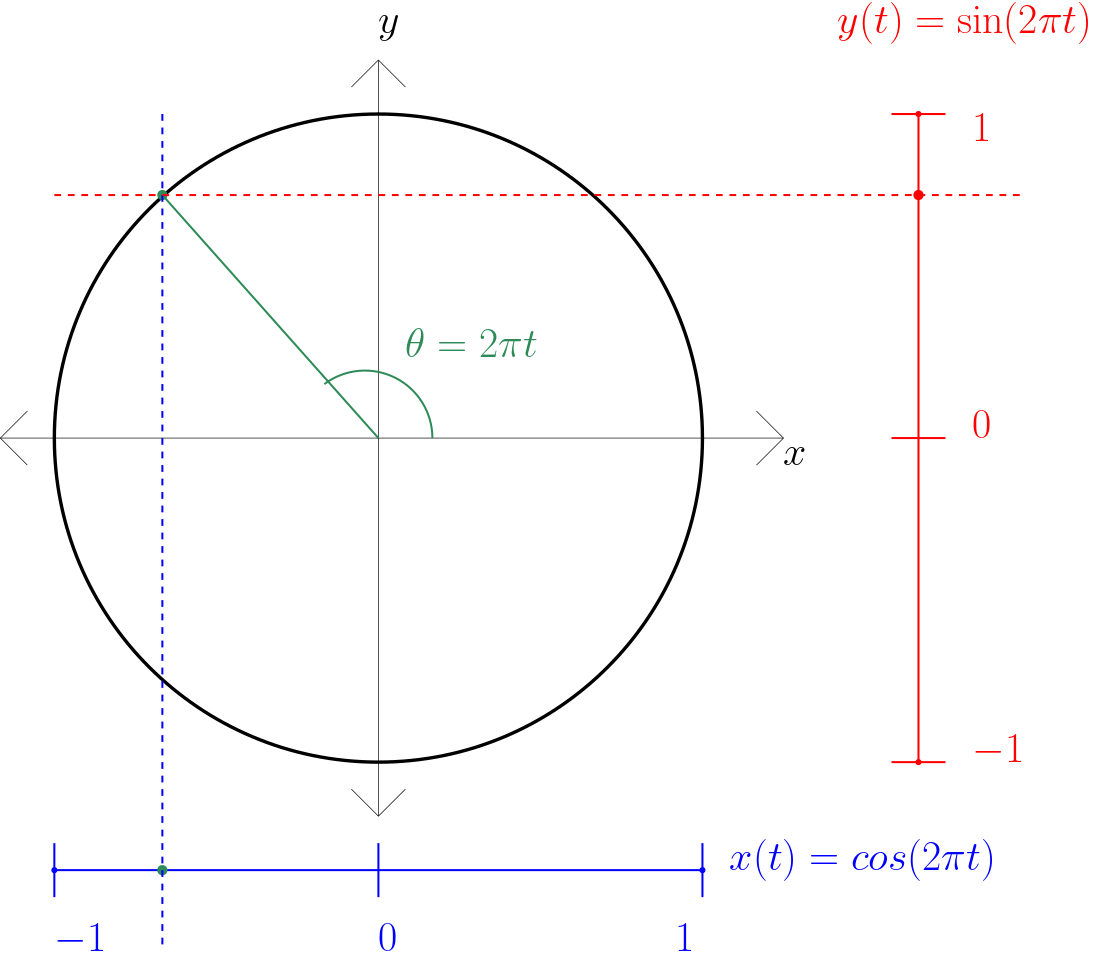
\includegraphics[width=.7\textwidth]{unitCircle.png}
    \caption{Simple example of the general idea in rendering a graphic using periodic functions on the Cartesian Plane. Figure produced using "Ipe" \protect\cite{IpeExtensibleDrawing}}
    \label{fig:unitCircle}
\end{figure}

\subsection{Enriched application to draw on the Argand Plane} \label{sec:big_guy}

In Section \ref*{sec:overarchingIdea}, it was explained that the overarching idea
of Fourier Series is to represent any periodic function as a sum of
sinusoidal functions. In Section \ref*{sec:cartplane}, the general
approach to rendering a graphic through periodic functions was discussed,
using the unit circle as an example. Recall that the final goal
is to render a graphic using Fourier Series on the Argand Plane,
meaning that a connection must be made between complex numbers and
the idea discussed in Section \ref*{sec:cartplane}. Fortunately,
Euler's formula as defined in Equation \ref*{eq:euler} will provide the strong link between
complex numbers and the idea surrounding rendering a graphic
using the Fourier Series.

\begin{equation}
    e^{it} = \cos(t) + i\sin(t)
    \label{eq:euler}
\end{equation}

For some value of \(t\), Euler's formula, when graphed on the Argand Plane,
will appear as a point where its position along the horizontal (real) axis
will equal to the real component of \(e^{it}\) which is \(\cos (t)\) and its
position along the vertical (imaginary) axis will equal to the imaginary
component of \(e^{it}\) which is \(i \sin (t)\). It therefore becomes
evident that Euler's formula manifests the same idea shown in Figure \ref*{fig:unitCircle} of moving
a point on a 2 dimensional plane according to a periodic function of time
indicating the point's position on the x-axis and another periodic
function of time indicating the point's position on the y-axis.

Before proceeding, recall that \(2\pi\) was multiplied within
both sinusoidal functions of \(y(t) = \sin (2\pi t)\)
and \(x(t) = \cos (2\pi t)\) in Section \ref*{sec:cartplane}
such that both periodic functions had a period of 1
to satisfy the restraint that \(t \in [0, 1]\).
This restraint still applies, therefore \(2 \pi\)
must be incorporated to Euler's formula as well
as shown below.

\begin{equation}
    e^{2\pi it} = \cos(2\pi t) + i\sin(2\pi t)
    \label{eq:2pi}
\end{equation}

For a complicated graphic,
it is easier to think of Euler's formula to be a rotating vector on the
Cartesian Plane or the
Argand Plane \cite{sandersonWhatFourierSeries2019}.
For the Cartesian Plane, each vector would be a grouping of one
sinusoidal term of the Fourier Series representing \(x(t)\)
and one sinusoidal term of the Fourier Series representing \(y(t)\),
with the amplitudes of the two grouped terms equal to eachother. This would mean
that the initial angle of standard position of the vector will not
always be 0 as if they were all 0, then the graphic must begin
on the x-axis with a positive \(x\) value. The reason behind
this varying initial angle will be explored more definitively later on
in the section; however, the factor that is important to consider
is that this will mean a phase shift of the sinusoidal
terms of \(x(t)\) and \(y(t)\) that is accomplished by
the inclusion of both sine and cosine terms in Equation \ref*{eq:sincos_form}.
This means that for a rotating vector modelled by Euler's formula,
there must be variable(s) that allow the definition of both
the amplitude of the vector and the initial angle in standard
position of the vector.

This will be accomplished by the variable \(c_n\), where \(n\) is the frequency
of revolution of the rotating vector,
which will be incorporated into Equation \ref*{eq:2pi} to get \(c_n e^{n \cdot 2\pi it}\). This will not
only allow for the vector to be scaled but also for the starting rotation of
the vector to be defined. Let's temporarily define \(c_n\) to be:

\begin{equation*}
    c_n = A \cdot z
\end{equation*}

\(A\) will indicate the factor to which the vector will be scaled by. Because
the original length of the vector was 1, then the factor will directly indicate
the length of the vector.

\(z\) will indicate the starting rotation of the vector, which would be
\(e^{i\theta}\), where \(\theta\) is the starting rotation angle in radians.

Lastly, it is important to note that when using Euler's formula for
Fourier series, \(n \in \mathbb{Z}\).
In the sine-cosine form of Fourier Series in Equation \ref*{eq:sincos_form},
\(n\) was defined by \(n \in \mathbb{N}\).
Returning to the idea surrounding a grouping of two sinusoidal terms
associated with the horizontal and vertical axes separately to create
a rotating vector,
then a vector that rotates clockwise can be achieved
by a particular mixture of parameters between the two
sinusoidal functions (e.g. \(x(t) = cos(2\pi t)\), \(y(t) = sin(-2\pi t) = -sin(2\pi t)\)).
This gives the reason behind why a negative values of \(n\) are not
necessary in the sine-cosine form of Fourier Series. However,
negative \(n\) values are necessary to include for Euler's formula,
as only the sign on the \(n\) value is capable of defining the direction
of rotation in Euler's formula.
\\

It could be imagined that the final Fourier Series that produces a desired drawing
is the sum of multiple vectors of different magnitudes rotating at different frequencies
indicated by \(n, n \in \mathbb{Z}\). Therefore, if \(f(t)\) is defined to be the
function that represents the drawing, this can be expressed mathematically
as:

\begin{equation}
    f(t) = \sum_{n=-\infty}^{\infty} c_n e^{n \cdot 2\pi it}
    \label{eq:ft_def}
\end{equation}

The main concern is how the value of \(c_n\) will be determined
for a specific drawing.

The easiest way to start off is by first considering \(c_0 e^{0 \cdot 2\pi it}\).
This can be simplified into \(c_0\), but what does this mean?
This is the vector that is rotating at a frequency of 0, which means that
it is static. It can therefore be defined to be the "centre of mass"\cite{sandersonWhatFourierSeries2019}
of the entire function.

If we take discrete intervals of \(t\) and obtain the value of \(f(t)\),
then by taking the average of all those values, we obtain a complex number
close to \(c_0\). This is illustrated by Figure \ref{fig:cnot_integ}.

\begin{figure}[H]
    \centering
    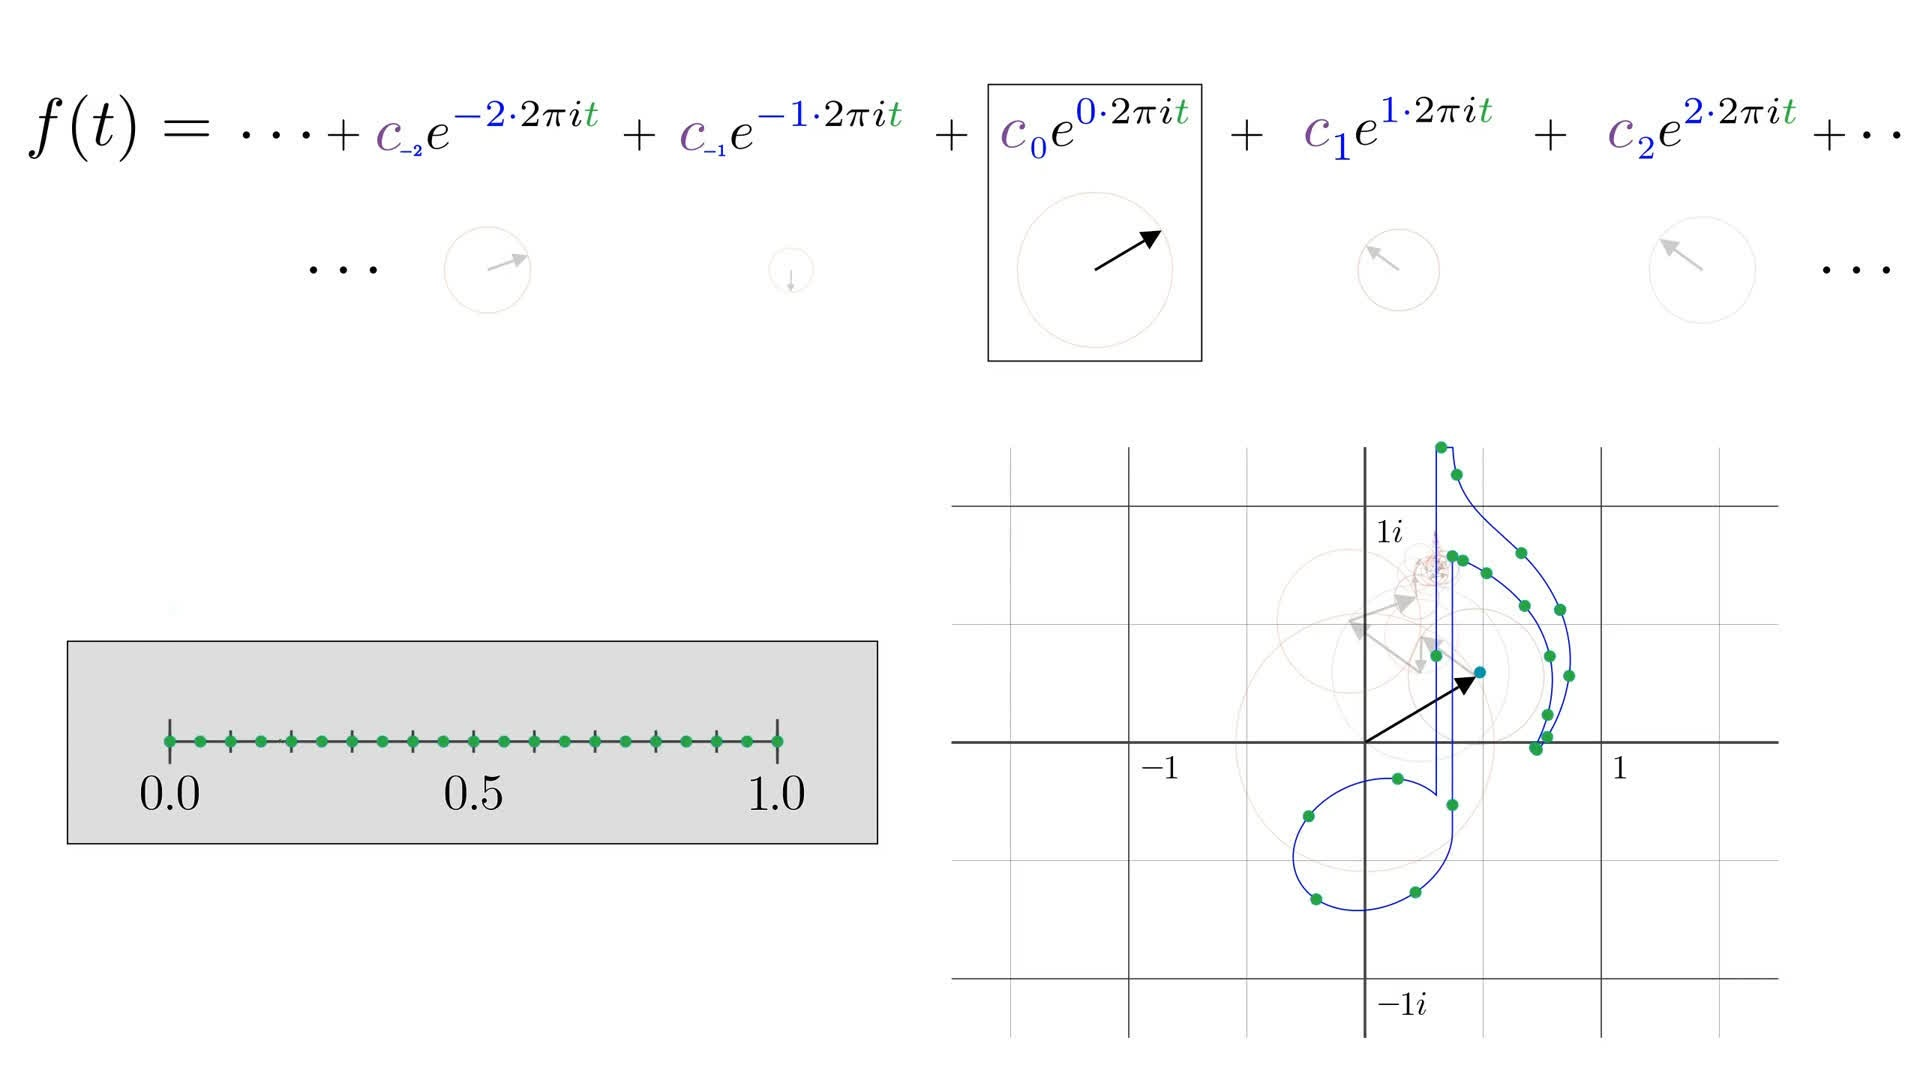
\includegraphics[width=\textwidth]{cnot_integ.jpeg}
    \caption{Averaging points throughout \protect\(f(t)\) illustrated \protect\cite{sandersonWhatFourierSeries2019}. The number line represent \protect\(t\), and the red dots on the musical note represent the resulting values of \protect\(f(t)\)}
    \label{fig:cnot_integ}
\end{figure}

With finer and finer intervals of \(t\), the result
becomes more and more accurate to the value of \(c_0\), therefore it can be
said that:

% TODO: Elaborate on how you derived the equation below
\begin{equation}
    c_0 = \lim_{\Delta t \to 0} \sum_{t = 0}^{\frac{1}{\Delta t}} f(t \cdot \Delta t) \Delta t
    \label{eq:cnot_lim}
\end{equation}

From Equation \textbf{(\ref*{eq:cnot_lim})}, \(c_0\) can ultimately be expressed as:

\begin{equation}
    c_0 = \int_{0}^{1} f(t) \,dt
    \label{eq:cnot_integ}
\end{equation}


We can use the same technique for all other values of \(n\), but the problem is
for all other values of \(n\) that are not 0, the vector is rotating, therefore
it doesn't make sense to take the average of the rotating vector.

Recalling the thorough definition of \(f(t)\) stated earlier in Equation \ref*{eq:ft_def},
we can substitute Equation \ref*{eq:ft_def} into Equation \ref*{eq:cnot_integ}.

\begin{align*}
     & c_0 = \int_{0}^{1} \sum_{n=-\infty}^{\infty} c_n e^{n \cdot 2\pi it} \,dt
    \\
     & c_0 = \int_{0}^{1} \left( \cdots + c_{-1} e^{-1 \cdot 2\pi it} + c_{0} e^{0 \cdot 2\pi it} + c_{1} e^{1 \cdot 2\pi it} + \cdots \right) \,dt
    \\
     & c_0 = \cdots + \int_{0}^{1} c_{-1} e^{-1 \cdot 2\pi it} \,dt + \int_{0}^{1} c_{0} e^{0 \cdot 2\pi it} \,dt + \int_{0}^{1} c_{1} e^{1 \cdot 2\pi it} \,dt + \cdots
\end{align*}

Remember that \(\int_{0}^{1} c_{0} e^{0 \cdot 2\pi it} \,dt\) was easy to simplify
as the power cancels out from being raised to 0. In turn, it can be further
evaluated to be just \(c_0\), as shown below:

\begin{align*}
     & \int_{0}^{1} c_{0} e^{0 \cdot 2\pi it} \,dt
    \\
     & = \int_{0}^{1} c_{0} \,dt
    \\
     & = c_{0}t]_{0}^1
    \\
     & = c_{0}
\end{align*}

Additionally, if all the other integrals were thought of as the the average of all
the points produced when its vector rotates by one revolution, then it can
be argued that each integral, when evaluated, would be 0.

This idea is illustrated in Figure \ref*{fig:circle_integ}.

\begin{figure}[H]
    \centering
    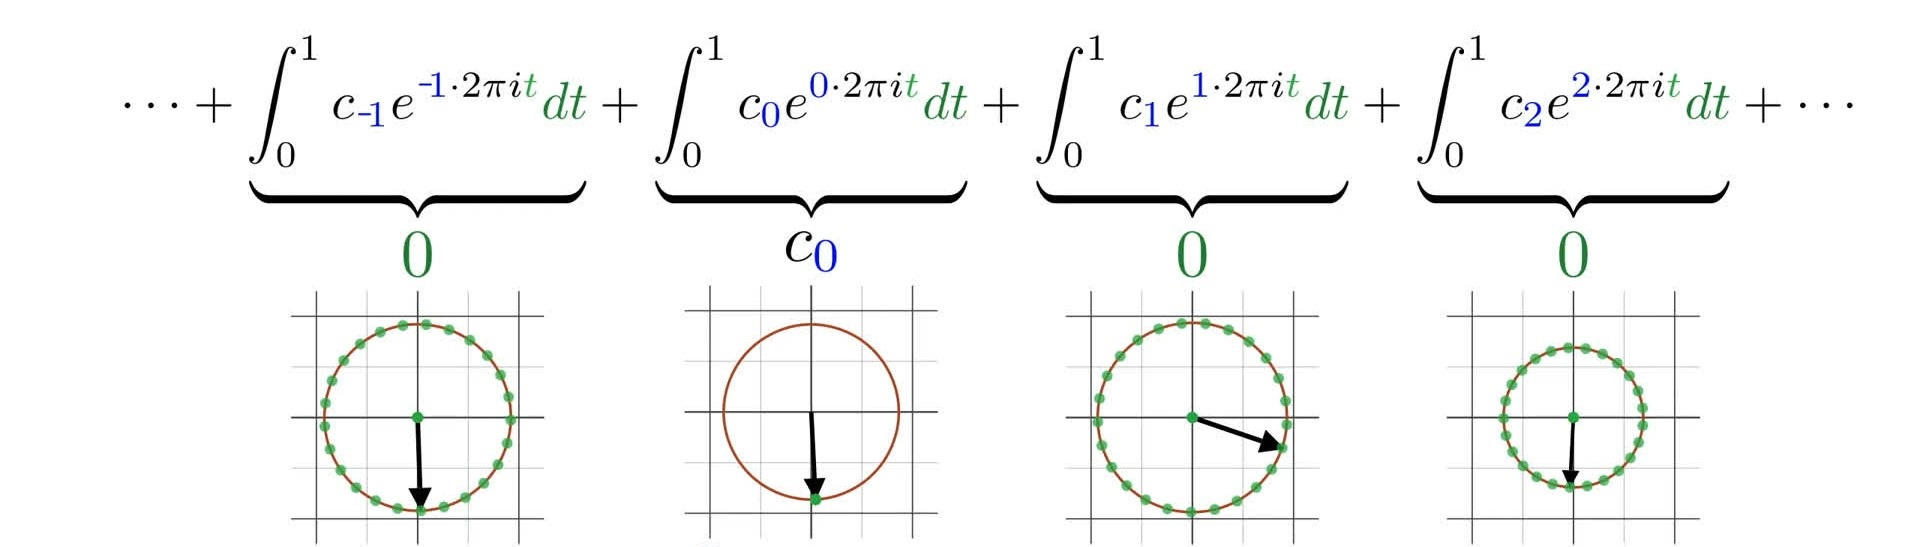
\includegraphics[width=\textwidth]{circle_integ.jpeg}
    \caption{Illustration of averaging all the points on a circle \protect\cite{sandersonWhatFourierSeries2019}.}
    \label{fig:circle_integ}
\end{figure}

If we were to multiply \(f(t)\) by \(e^{-n \cdot 2\pi it}\), then an effect can occur
where all of the power's exponents will decrease by \(n\). Ultimately, we will
get a similar scenario in the summation of all the integrals where
all integrals are evaluated to become 0 except for the integral
where \(n = 0\), which evaluates to \(c_0\). However, the multiplication
of the two powers will cause the integral of some \(n\) value to simplify to just
\(c_n\).

This mechanism is mathematically shown below.
\begin{align*}
     & n = 1
    \\
     & c_1 = \int_{0}^{1} f(t) e^{-1 \cdot 2\pi it} \,dt
    \\
     & c_1 = \cdots + \int_{0}^{1} c_{-1} e^{-1 \cdot 2\pi it} \cdot e^{-1 \cdot 2\pi it} \,dt
    \\
     & + \int_{0}^{1} c_{0} e^{0 \cdot 2\pi it} \cdot e^{-1 \cdot 2\pi it} \,dt + \int_{0}^{1} c_{1} e^{1 \cdot 2\pi it} \cdot e^{-1 \cdot 2\pi it} \,dt + \cdots
    \\
     & c_1 = \cdots + \int_{0}^{1} c_{-1} e^{-2 \cdot 2\pi it} \,dt + \int_{0}^{1} c_{0} e^{-1 \cdot 2\pi it} \,dt + \int_{0}^{1} c_{1} e^{0 \cdot 2\pi it} \,dt + \cdots
    \\
     & c_1 = \cdots + 0 + 0 + c_1 + 0 + 0 + \cdots
    \\
     & c_1 = c_1
\end{align*}

Therefore, \(c_n\) can be defined as:

\begin{equation}
    c_n = \int_{0}^{1} f(t) e^{-n \cdot 2\pi it} \,dt
    \label{eq:cn_integ}
\end{equation}

Equation \ref*{eq:cn_integ} is what will be used in order to
determine each value of \(c_n\)
\\

All concepts of this section come from \cite{sandersonWhatFourierSeries2019}.


\subsection{Bézier curves}

\subsubsection{Linear interpolation}

Suppose there is a free moving point \(P\) on the line drawn between
the stationary points \(P_0\) and \(P_1\) as illustrated on
Figure \ref*{fig:2_point_bezier}.

\begin{figure}[H]
    \centering
    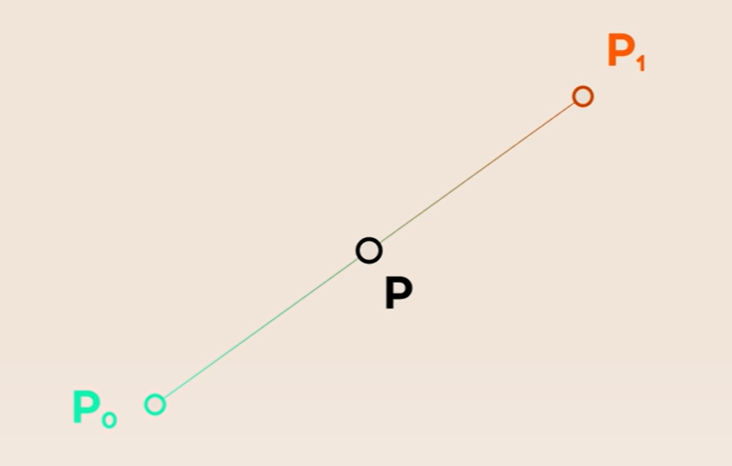
\includegraphics[width=.8\textwidth]{2_point_bezier.png}
    \caption{2 point Bézier \protect\cite{holmerBeautyBezierCurves2021}.}
    \label{fig:2_point_bezier}
\end{figure}

The position of \(P\) along the line will be defined by \(t\), which
is thought of to be the percentage that \(t\) is along the line,
where \(t = 100\%\) is located at \(P_1\) and \(t = 0\%\) is located
at \(P_0\). This process is called linear interpolation (lerp) and
can be expressed mathematically as:

\begin{equation}
    P = lerp(P_0, P_1, t) = (1-t)P_0 + tP_1
    \label{eq:lerp_def}
\end{equation}
where \(lerp(P_0, P_1, t)\) is the function that represents the
process of lerping.


\subsubsection{Cubic Bézier curves}

While there are many types of Bézier curves, this investigation will
only focus on Cubic Bézier curves as they are the only type of Bézier curve used in the IB Logo.

Suppose that instead of just 2 points, there are 4 points on the
plane (\(P_0, P_1, P_2, P_3\)). The lines are drawn so that
\(P_0\) connects to \(P_1\), \(P_1\) connects to \(P_2\), and
\(P_2\) connects to \(P_3\) such that \(P_0\) and \(P_3\) are both
endpoints.

Each line segment has its own individual moving point, with all moving
points "lerping" according to the same universal \(t\) value.

Lines can then be drawn between these new moving points, and
these points lerp according to the same \(t\) value.

This process of adding points on lines and drawing new lines
until just one moving point along a single line is created, which
will be the "pen" of the Bézier curve.

This is all illustrated by Figures \ref*{fig:cubic_ill_mid} and \ref*{fig:cubic_ill_end}.

\begin{figure}[H]
    \centering
    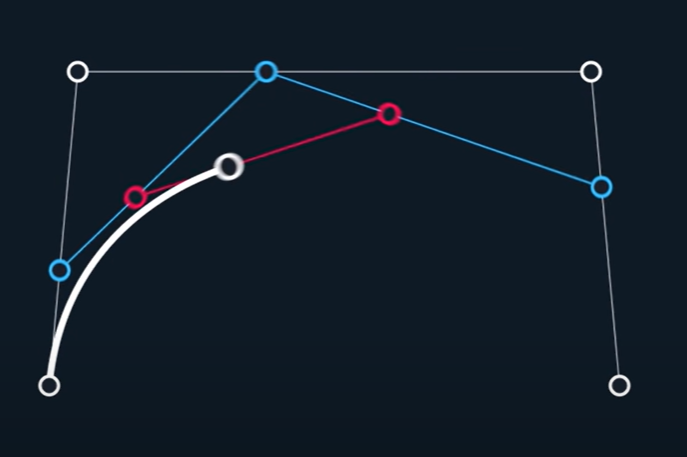
\includegraphics[width=.8\textwidth]{cubic_ill_mid.png}
    \caption{Cubic Bézier around the middle of its lerp \protect\cite{holmerBeautyBezierCurves2021}.}
    \label{fig:cubic_ill_mid}
\end{figure}

\begin{figure}[H]
    \centering
    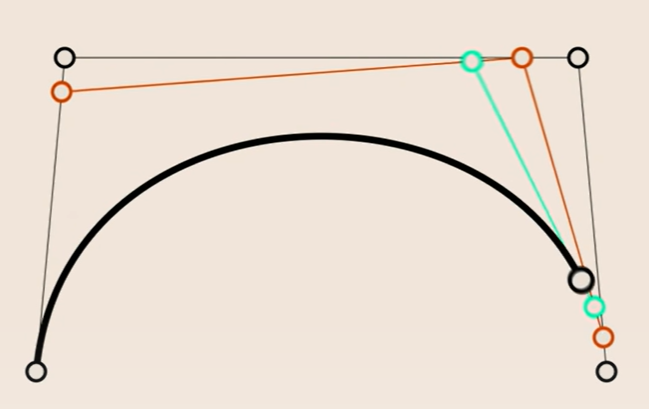
\includegraphics[width=.8\textwidth]{cubic_ill_end.png}
    \caption{Cubic Bézier nearing the end of its lerp \protect\cite{holmerBeautyBezierCurves2021}.}
    \label{fig:cubic_ill_end}
\end{figure}

\subsubsection{Bernstein Polynomial Form}

\begin{figure}[H]
    \centering
    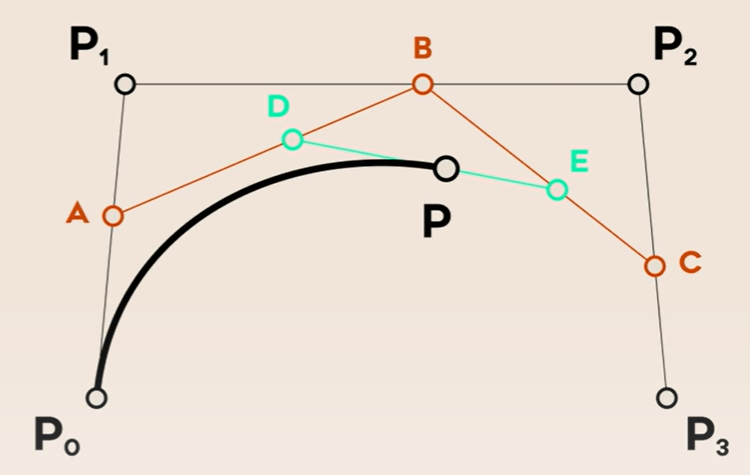
\includegraphics[width=.8\textwidth]{labelled_cubic.png}
    \caption{Cubic Bézier curve with labelled points \protect\cite{holmerBeautyBezierCurves2021}.}
    \label{fig:labelled_cubic}
\end{figure}

We can derive a general formula for \(P\) in terms of \(P_0, P_1, P_2, P_3, t\) by expanding out
all of the lerp functions for each point in a Cubic Bézier curve
and substituting when necessary, as shown below. Variables are
with reference to Figure \ref*{fig:labelled_cubic}.

\begingroup
\allowdisplaybreaks
\begin{align*}
     & A = lerp(P_0, P_1, t)
    \\
     & B = lerp(P_1, P_2, t)
    \\
     & C = lerp(P_2, P_3, t)
    \\
     & D = lerp(A, B, t)
    \\
     & E = lerp(B, C, t)
    \\
     & P = lerp(D, E, t)
    \\
    \\
     & \text{From Equation } \protect\ref*{eq:lerp_def}
    \\
     & lerp(P_0, P_1, t) = (1-t)P_0 + tP_1
    \\
    \\
     & A = (1-t)P_0 + tP_1
    \\
     & B = (1-t)P_1 + tP_2
    \\
     & C = (1-t)P_2 + tP_3
    \\
     & D = (1-t)A + tB
    \\
     & E = (1-t)B + tC
    \\
     & P = (1-t)D + tE
    \\
    \\
     & P = P_0(-t^3+3t^2-3t+1) + P_1(3t^3-6t^2+3t)
    \\
     & + P_2(-3t^3+3t^2) + P_3(t^3)
\end{align*}
\endgroup

Therefore, the general formula for \(P\) in terms of
\(P_0, P_1, P_2, P_3, \text{and} t\) is

\begin{equation} \label{eq:pFormula}
    P = P_0(-t^3+3t^2-3t+1) + P_1(3t^3-6t^2+3t) + P_2(-3t^3+3t^2) + P_3(t^3)
\end{equation}

All information regarding Bézier curves come from \cite{holmerBeautyBezierCurves2021}.

\subsection{Composition of ".svg" files}

SVG files are "XML-based vector image format for defining two dimensional
graphics"\cite{SVG2023}.

An SVG's two dimensional size is defined by the "viewBox" attribute,
which will indicate the width and height of the canvas.

There are many attributes for drawing predefined shapes, but what
we are concerned with is the "path" attribute, which allows for custom
shapes and is what the IB logo will be composed of.

The "path" attribute will be defined by various curves that are indicated
by letters. The letters that are of concern in this investigation are
listed below.
\begin{itemize}
    \item M: Move the pen to somewhere without drawing a line
    \item C: Cubic Bézier defined by the starting location, 2 control points, and an indicated end location
    \item L: Draw a vertical line to some coordinate
    \item V: Draw a vertical line up to some y-coordinate
    \item Z: Draw a straight line back to the first point of the path
\end{itemize}

Note that when the letter is lowercase, the coordinates specified will
be relative to the current position (ex. \(m~\Delta x~\Delta y\)). If the letter is uppercase, the
coordinates specified will be absolute to the canvas (ex. \(M~x~y\)).

All information regarding paths come from \cite{mozilladevelopernetworkPathsSVGScalable2023}.




\section{Calculation and Computation}

\subsection{Analysis of the ".svg" File} \label{svgAnalysis}

On a canvas of height 198.426px and width 198.425px,
a few lines of the path of the IB Logo is presented below,
with the entire path presented in Section \ref*{app:fullSVG}
of the appendix
\cite{internationalbaccalaureateorganisationInternationalBaccalaureateLogo2013}. \textbf{Note: SVG files interpret positive y-values as downwards.}

\begin{verbatim}
    <path fill="url(#SVGID_1_)" d="
    M198.425,99.155
    c 0,54.833 -45.075,99.271 -100.685,99.271
    c -47.27, 0 -86.91 -32.11 -97.74 -75.416
    c 19.703 -0.222, 38.391 -4.567, 55.26 -12.149
    V 72.226
    ...
    C 68.199, 48.705, 71.582, 47.359, 74.363, 44.669
    z"/>
\end{verbatim}

Disregarding any "Move" actions, there are 54 pen strokes
in total for the IB Logo. This means that for the starting piecewise
form of \(f(t)\), each piece will have a domain of \(\frac{1}{54}(n-1) \le t < \frac{1}{54}n\),
where \(n\) represents the index of the current pen stroke.

The contents of this path was moved into an Excel Spreadsheet for
the sake of organization, with part of the spreadsheet shown
in Figure \ref*{fig:svgxlsx}.

\begin{figure}[H]
    \centering
    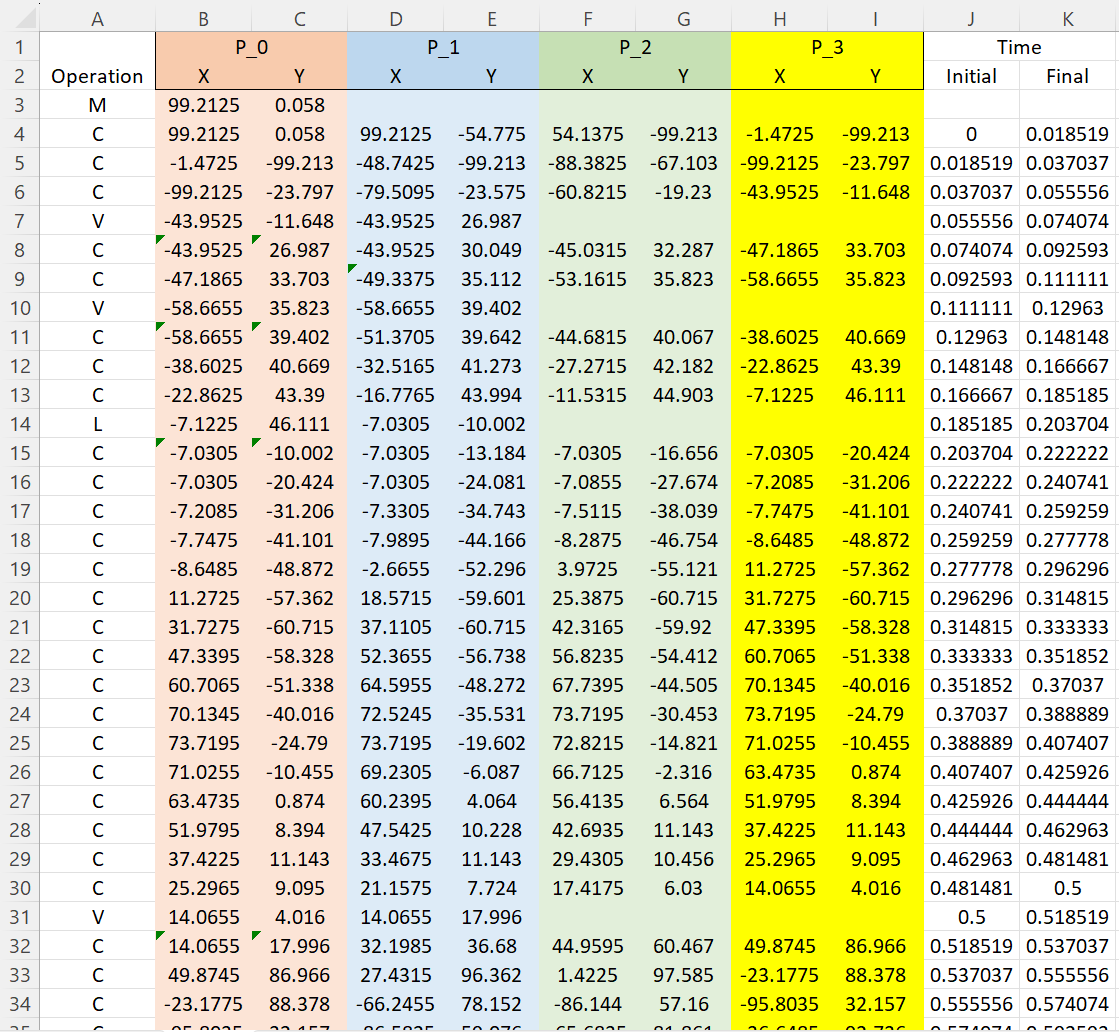
\includegraphics[width=0.8\textwidth]{svgxlsx.png}
    \caption{Path data imported in an Excel Spreadsheet}
    \label{fig:svgxlsx}
\end{figure}

Using Javascript under the NodeJS Runtime, this spreadsheet can
be read using the NPM Package "read-excel-file" \cite{kuchumovReadexcelfile}.
This package will parse the spreadsheet into an array of rows,
with each row being an array of cells. Then, the code presented
below will iterate through each row, with access to all the cells
in that row indexed by zero-based numbering.

\begin{lstlisting}[language=JavaScript]
    readXlsxFile('./SVG_Coordinate_Spreadsheet.xlsx')
    .then((rows) => {
        // `rows` is an array of rows
        // each row being an array of cells.
        rows.forEach(row => {
            // iterate through each row, accessing the
            // cells of each row
        });
    })
\end{lstlisting}

For each row, the code checks if the operation for the current
row is relevant for drawing. Only "Move" (M) is ignored, and
all "Z" operations were written down as "line" (L) operations.
Using the data within each row, the parameter of \(c_n\) can be
computed for each value of \(n\).

\subsection{Computation of parameters}

Given that \(f(t)\) is able to be determined as a piecewise function
from the previous section, the desired summation representing
\(f(t)\) can be determined.

Referring back to Section \ref*{sec:big_guy}, \(c_n\) is defined as:

\begin{equation*}
    c_n = \int_{0}^{1} f(t) e^{-n \cdot 2\pi it} \,dt
\end{equation*}

This means that every \(c_n\) must be determined individually. Therefore,
it becomes evident that it is unreasonable to evaluate the infinite sum of
\(f(t) = \sum_{n=-\infty}^{\infty} c_n e^{n \cdot 2\pi it}\), and that
the limits of the summation must be defined.

Let's rewrite \(f(t)\) as:
\begin{equation*}
    f(t) = \sum_{n=-k}^{k} c_n e^{n \cdot 2\pi it}
\end{equation*}

so that \(k\) indicates the selected frequency of the two fastest vectors
that are spinning in opposite directions to each other.

As \(k \to \infty\), \(f(t)\) becomes more and more accurate to
the original drawing, which will be demonstrated by performing distinct
analyses for various values of \(k\).

\subsubsection{Approach to integration} \label{sec:approachInteg}

\begin{equation*}
    c_n = \int_{0}^{1} f(t) e^{-n \cdot 2\pi it} \,dt
\end{equation*}

The integral above can be evaluated for some value of \(n\) by
taking some small value to represent \(\Delta t\), in which
by summing up the values from \(f(t) e^{-n \cdot 2\pi it}\)
produced by each increment of \(t\) by \(\Delta t\), a value close
to the original integral can be determined \cite{sandersonWhatFourierSeries2019}.
This is known as a Riemann Sum \cite{RiemannSum2023}.

\begin{equation}
    c_n = \sum_{t = 0}^{\frac{1}{\Delta t}} f(t \cdot \Delta t) e^{-n \cdot 2\pi i(t \cdot \Delta t)} \Delta t
    \label{eq:cn_riemann_sum}
\end{equation}

Because a small value of \(\Delta t\) must be used, \(c_n\) must
be evaluated through a computer. Additionally, since the original
version of \(f(t)\) can be thought of as a piecewise function composed
of Bézier curves and lines, then Equation \ref*{eq:cn_riemann_sum}
must be split up into multiple sums, each accounting for the domain
of each piece of the piecewise function (\(\frac{1}{54}(n-1) \le t < \frac{1}{54}n\)).
From this consideration, Equation \ref*{eq:cn_riemann_sum} can be
expressed as the following:

\begin{equation}
    \begin{aligned} \label{eq:riemann_Expanded}
         & c_n = \sum_{t = 0}^{(\frac{1}{54})(\frac{1}{\Delta t})} f(t \cdot \Delta t) e^{-n \cdot 2\pi i(t \cdot \Delta t)} \Delta t
        + \sum_{t = (\frac{1}{54})(\frac{1}{\Delta t})}^{(\frac{2}{54})(\frac{1}{\Delta t})} f(t \cdot \Delta t) e^{-n \cdot 2\pi i(t \cdot \Delta t)} \Delta t
        \\
         & + \cdots
        + \sum_{t = (\frac{53}{54})(\frac{1}{\Delta t})}^{(\frac{54}{54})(\frac{1}{\Delta t})} f(t \cdot \Delta t) e^{-n \cdot 2\pi i(t \cdot \Delta t)} \Delta t
    \end{aligned}
\end{equation}

Additionally, in order to evaluate the complete range of \(f(t)\)
for some section, \(f(t)\) must take in the complete domain of
\([0, 1]\). The reason for this will be elaborated on in
Section \ref*{sec:bezierCalc}, but because each section will only
account for the same domain defined by \([\frac{1}{54}(n-1), \frac{1}{54}n)\),
then \(f(t)\) must take an input of a manipulated value of \(t\).
To simplify this manipulation, let's make every summation in
Equation \ref*{eq:riemann_Expanded} have limits from 0 to
\(\frac{1}{54\Delta t}\) and add the initial time of each
section to \(t \cdot \Delta t\) in the expression
\(e^{-n \cdot 2\pi i(t \cdot \Delta t)}\) so that
the calculation for such expression stays absolute to the universal
time passage. The input of \(f(t)\) can therefore be multiplied
by 54 so that when the upper limit of the summation (\(\frac{1}{54\Delta t}\))
is multiplied by 54 and \(\Delta t\), then the resulting value
is 1 (\(\frac{1}{54\Delta t} \cdot 54\Delta t = 1\)).
This therefore offers a domain for \(f(t)\) from 0 to 1 even if
\(t \in [\frac{1}{54}(n-1), \frac{1}{54}n)\) for each
summation.


Overall, if we let \(f_n(t)\) equal to the function \(f(t)\) isolated
to just the \(n^{\text{th}}\) section,
Equation \ref*{eq:cn_riemann_sum} can
be expressed as:

\begin{equation}
    \begin{aligned} \label{eq:riemann_Codefriendly}
         & c_n = \sum_{t = 0}^{\frac{1}{54\Delta t}} f_1(54t \cdot \Delta t) e^{-n \cdot 2\pi i(t \cdot \Delta t + 0)} \Delta t
        \\
         & + \sum_{t = 0}^{\frac{1}{54\Delta t}} f_2(54t \cdot \Delta t) e^{-n \cdot 2\pi i(t \cdot \Delta t + \frac{1}{54})} \Delta t
        \\
         & + \sum_{t = 0}^{\frac{1}{54\Delta t}} f_3(54t \cdot \Delta t) e^{-n \cdot 2\pi i(t \cdot \Delta t + \frac{2}{54})} \Delta t
        \\
         & + \cdots +
        \sum_{t = 0}^{\frac{1}{54\Delta t}} f_{54}(54t \cdot \Delta t) e^{-n \cdot 2\pi i(t \cdot \Delta t + \frac{53}{54})} \Delta t
    \end{aligned}
\end{equation}

Therefore, the approach of the code will be to iterate through
each value of \(n\) from \(-k \le n \le k\), and evaluate
the Riemann Sum using Equation \ref*{eq:riemann_Codefriendly}.

The computer program saves a Dictionary composed of a searchable key,
which will composed of all of the possible \(n\) values within
a defined range that comes from a user input specifying what
\(k\) equals. Then, each key will have an associated value
that will start as being defined to be \(0 + 0i\), which
is achievable through the "complex" object offered by the
"mathjs" NPM package \cite{dejongMathjs}.

Then, for each row of the Excel Spreadsheet (in which the process of
iterating through every row was explained in Section \ref*{svgAnalysis}),
every possible value for \(n\) is analyzed with a for loop,
allowing the program to evaluate the value of \(c_n\) associated with
each row.
% TODO: find a way to incorporate the for loop code in here

The following code is equivalent to Equation \ref*{eq:riemann_Codefriendly}.
\textbf{Note: "f" represents f(t) and
    the calculation for it will differ based on whether
    a Bézier curve or a Straight Line is being drawn.
    The calculation for f(t) will be elaborated on in
    Section \ref*{sec:bezierCalc}.}

\begin{lstlisting}[language=JavaScript]
    for(let t = 0; t < 1/sectionCount/dt; t++){
        const f = null;
        const add = math.multiply(dt, math.multiply(f, math.pow(math.e, math.multiply(math.complex(0, 1), -2 * n * math.pi * (t * dt + row[9])))));
        CnDict[n] = math.add(CnDict[n], add);
    }
\end{lstlisting}

\subsubsection{Calculation for Cubic Bézier curves} \label{sec:bezierCalc}

Recalling that Equation \ref*{eq:pFormula} stated that

\begin{equation*}
    P = P_0(-t^3+3t^2-3t+1) + P_1(3t^3-6t^2+3t) + P_2(-3t^3+3t^2) + P_3(t^3)
\end{equation*}

This was originally meant for when \(P, P_0, P_1, P_2, P_3\)
were ordered pairs on a Cartesian Plane. However, because
multiplication between a scalar and a Cartesian Vector operates
similarly to multiplication between a scalar and a complex number,
then \(P_0, P_1, P_2, P_3\) are allowed to be expressed as complex
numbers. Given this condition, \(P\) would be equivalent to \(f(t)\)
because \(P\) is the Cartesian vector for all points defined
by a Bézier curve, and if the result representing \(P\) was a complex
number, then \(P\) is representable as a function of \(t\).

Something crucial to consider is that \(t\) in Equation \ref*{eq:pFormula}
is \textbf{not} the time passage in drawing the IB logo but rather
the lerp of the Bézier curve from 0 to 1. To distinguish this distinction,
the function will instead take in an input \(j\), with the relationship
between \(j\) and \(t\) being established in Section \ref*{sec:approachInteg}
to be \(j = 54t\).

Ultimately, the Bézier curve can be expressed as:

\begin{equation} \label{eq:f_of_j_Cubic}
    f(j) = P_0(-j^3+3j^2-3j+1) + P_1(3j^3-6j^2+3j) + P_2(-3j^3+3j^2) + P_3(j^3)
\end{equation}

The value of \(f(j)\) is evaluated through the
following code, which is equivalent to Equation \ref*{eq:f_of_j_Cubic}:

\begin{lstlisting}[language=JavaScript]
    const sectionCount = 54;

    function subTimeCalc(t){
        return sectionCount * t;
    };

    const fCubicCalc = (t, r) => {
        const P0 = math.complex(r[1], r[2]);
        const P1 = math.complex(r[3], r[4]);
        const P2 = math.complex(r[5], r[6]);
        const P3 = math.complex(r[7], r[8]);

        let j = subTimeCalc(t);
        const ret = 
            math.add(
                math.add(
                    math.multiply(P0, (-1*math.pow(j,3) + 3*math.pow(j,2) - 3*j + 1)),
                    math.multiply(P1, (3*math.pow(j,3) - 6*math.pow(j,2) + 3*j))
                ),
                math.add(
                    math.multiply(P2, (-3*math.pow(j,3) + 3*math.pow(j,2))),
                    math.multiply(P3, (math.pow(j,3)))
                )
            )
        return ret;
    };
\end{lstlisting}

\subsubsection{Calculation for Straight Lines}

In Section \ref*{sec:bezierCalc}, it was mentioned that \(t\) cannot
be used as the input of \(f(t)\) as the original meaning of \(t\) in
such context was the lerp progression in the Bézier curve.

While \(t\) could be used in the calculation of \(f(t)\) for straight lines,
it is actually better to continue to use \(j = 54t\), as this allows
for consistency and will make the derived equations relevant in the section
to be way cleaner than if \(t\) was used.

Every line will have an initial point at \(j=0\) that can be
expressed as \(x_0 + iy_0\), as well as a final point at \(j=1\)
that can be expressed as \(x_1 + iy_1\).

Because the pathway between these two points is a straight line,
then two linear functions can be found for \(x\) and \(y\) that
are in terms of \(j\). This means that \(f(j)\) can be expressed
as follows:

\begin{equation*}
    f(j) = x(j) + iy(j)
\end{equation*}

The formula for \(x(j)\) is derived below.

\begin{align*}
     & x(j) = mj + b
    \\
     & b = x_0
    \\
     & m = \frac{\Delta x}{\Delta j}
    \\
     & = \frac{x_1 - x_0}{1 - 0}
    \\
     & = x_1 - x_0
    \\
     & x(j) = (x_1 - x_0)j + x_0
\end{align*}

\(y(j)\) can be said to have a similar formula, as \(x_0, x_1\) are
simply replaced by \(y_0, y_1\), and \(\Delta j\) remains 1.

Ultimately, \(f(j)\) can be expressed as follows:

\begin{equation}
    f(j) = ((x_1 - x_0)j + x_0) + i((y_1 - y_0)j + y_0)
\end{equation}

This is evaluated through the following code:
\begin{lstlisting}[language=JavaScript]
    const f =
    math.add(
        math.add(
            row[1],
            math.multiply(
                subTimeCalc(t * dt),
                row[3] - row[1]
            )
        ),
        math.multiply(
            math.complex(0, 1),
            math.add(
                row[2],
                math.multiply(
                    subTimeCalc(t * dt),
                    math.add(
                        row[4],
                        -1 * row[2]
                    )
                )
            )
        )
    );
\end{lstlisting}

\subsection{Rendering the final image}

Recalling that the end result of \(f(t)\) is defined as the equation
below, then rendering the final image is just a matter of going
through various values of \(t\), summing up \(c_n e^{n \cdot 2\pi it}\)
for all values of \(k\), and rendering the result by placing
the real parts of \(f(t)\) on the horizontal axis on a plane,
and placing the imaginary part of \(f(t)\) on the vertical axis
on a plane.

\begin{equation*}
    f(t) = \sum_{n=-k}^{k} c_n e^{n \cdot 2\pi it}
\end{equation*}

Because all possible \(n\) values within an given domain and
their associated values for \(c_n\) were stored in a dictionary,
then iterating through the dictionary will allow for accessing
all of the \(c_n\) values properly linked with their associated \(n\) value.

The code that calculates \(f(t)\) and renders the result is presented below:
\begin{lstlisting}[language=JavaScript]
    let universalTime = 0;

    function plotPoint(x, y){
        const adjX = x + 99.2125;
        const adjY = -y + 99.213;
        ctx.strokeStyle = 'rgba(255,0,0,1)';
        ctx.beginPath();
        ctx.lineTo(adjX-1, adjY);
        ctx.lineTo(adjX+1, adjY);
        ctx.stroke();
    }

    function finalF(){
        while(universalTime <= 1){
            let curr = math.complex(0, 0);
            Object.entries(CnDict).forEach(pair => {
                [currN, cn] = pair;
                //for a specific time
                //calculate f(t)
                //plot
                curr = math.add(
                    curr,
                    math.multiply(
                        cn,
                        math.pow(
                            math.e,
                            math.multiply(
                                math.complex(0, 1),
                                currN * 2 * math.pi * universalTime
                            )
                        )
                    )
                )
            });
            plotPoint(curr.re, curr.im);
            universalTime += dt;
        }
    }

    finalF();
    console.log('<img src="' + canvas.toDataURL() + '" />');
\end{lstlisting}

\section{Results}

\begin{figure}[H]
    \centering
    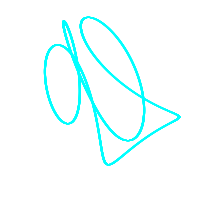
\includegraphics[width=.5\textwidth]{5.png}
    \caption{\protect\(\Delta t = 0.0001, k = 5\), 10 spinning vectors, 11 total vectors}
    % \label{fig:svgxlsx}
\end{figure}

\begin{figure}[H]
    \centering
    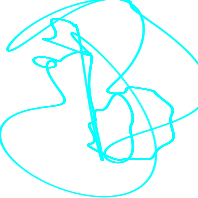
\includegraphics[width=.5\textwidth]{25.png}
    \caption{\protect\(\Delta t = 0.0001, k = 25\), 50 spinning vectors, 51 total vectors}
    % \label{fig:svgxlsx}
\end{figure}

\begin{figure}[H]
    \centering
    
\includegraphics[width=.5\textwidth]{1000.png}
    \caption{\protect\(\Delta t = 0.00001, k = 1000\), 2000 spinning vectors, 2001 total vectors}
    % \label{fig:svgxlsx}
\end{figure}

\section{Conclusion}

Throughout this investigation, the aim of converting
the IB logo into a Fourier Series and in turn
rendering the IB logo using its Fourier Series has been
accomplished. In addition to that, connecting
Fourier Series with complex numbers has enabled
the ability to handle a two-dimensional
logo without separating it into two components.

The primary limitation with my approach to this investigation
was the inflexibility in terms of what the
computer program could convert into a Fourier Series.
Ideally, the program should take in a ".svg" file and
automatically convert the path to Bézier curves
as representation of what \(f(t)\) is
prior to being converted to a Fourier Series.
This is all due to transferring all the values
to an Excel spreadsheet, which makes it easier to
see the moving parts but prevents the program
from analyzing any kind of vector art
without the conversion of an ".svg" file into
a spreadsheet and modifications to the code
(e.g. number of Bézier curves or lines, size of canvas).

Another limitation is that the method of
going through the ".svg" path without
considering continuity resulted in the artifacts present
in the final result. This may be
prevented in a future investigation
by coding a program to begin
parsing a separate \(f(t)\) function
after detection of a significant and sudden
change between the previous and current
complex values.

I expect that I will be able to handle learning
Fourier Series in some university course
in the future with ease. Although it is likely
that Fourier Series will be taught in a course
in the context of real numbers using
\(\sin(t)\) and \(\cos(t)\) instead of \(e^{it}\),
the same mechanisms will still be present around
determining the coefficients for each term of
the series, which has been the largest hurdle
for me in comprehending Fourier Series in this
investigation.

The main area of extension of this investigation
is the way in which the integral for \(c_n\) was
evaluated where it was evaluated as a Riemann Sum.
It is possible to evaluate this integral through
integration by parts; however, the challenge
when incorporating this into the method of this investigation
is that because each Bézier curve is evaluated
between 0 and 1, then numerous integrals
must be evaluated with a unique transformation
to each Bézier curve piece part of the original
piece-wise \(f(t)\) function thereby resulting
in more and more complicated integrals
for pieces of the function nearing the end boundary.

\bibliographystyle{apacite}
\bibliography{IB_MATH_IA.bib}

\appendix

\section{Full SVG Path} \label{app:fullSVG}

\begin{verbatim}
    <path fill="url(#SVGID_1_)" d="
    M198.425,99.155
    c 0,54.833 -45.075,99.271 -100.685,99.271
    c -47.27, 0 -86.91 -32.11 -97.74 -75.416
    c 19.703 -0.222, 38.391 -4.567, 55.26 -12.149
    V 72.226
    c 0 -3.062 -1.079 -5.3 -3.234 -6.716
    c -2.151 -1.409 -5.975 -2.12 -11.479 -2.12
    v -3.579
    c 7.295 -0.24, 13.984 -0.665, 20.063 -1.267
    c 6.086 -0.604, 11.331 -1.513, 15.74 -2.721
    l 0.092, 56.113
    c 0, 3.182, 0, 6.654, 0, 10.422
    c 0, 3.657 -0.055, 7.25 -0.178, 10.782
    c -0.122, 3.537 -0.303, 6.833 -0.539, 9.895
    c -0.242, 3.065 -0.54, 5.653 -0.901, 7.771
    c 5.983, 3.424, 12.621, 6.249, 19.921, 8.49
    c 7.299, 2.239, 14.115, 3.353, 20.455, 3.353
    c 5.383, 0, 10.589 -0.795, 15.612 -2.387
    c 5.026 -1.59, 9.484 -3.916, 13.367 -6.99
    c 3.889 -3.066, 7.033 -6.833, 9.428 -11.322
    c 2.39 -4.485, 3.585 -9.563, 3.585 -15.226
    c 0 -5.188 -0.898 -9.969 -2.694 -14.335
    c -1.795 -4.368 -4.313 -8.139 -7.552 -11.329
    c -3.234 -3.19 -7.06 -5.69 -11.494 -7.52
    c -4.437 -1.834 -9.286 -2.749 -14.557 -2.749
    c -3.955, 0 -7.993, 0.687 -12.126, 2.048
    c -4.139, 1.371 -7.879, 3.065 -11.231, 5.079
    V 81.217
    c 18.133 -18.684, 30.894 -42.471, 35.809 -68.97
    c -22.443 -9.396 -48.452 -10.619 -73.052 -1.412
    C 32.967, 21.061, 12.981, 42.053, 3.409, 67.056
    c 9.221 -26.919, 30.12 -49.704, 59.155 -60.579
    c 24.245 -9.068, 49.573 -8.27, 71.696, 0.248
    c 0.002 -0.021, 0.011 -0.045, 0.014 -0.063
    C 171.81, 21.082, 198.425, 57.046, 198.425, 99.155
    z 
    M 100.598, 149.993
    c 2.746, 4.661, 7.408, 6.986, 13.987, 6.986
    c 6.564, 0, 11.233 -2.325, 13.985 -6.986
    c 2.749 -4.652, 4.123 -11.988, 4.123 -22.013
    c 0 -10.014 -1.374 -17.353 -4.123 -22.008
    c -2.752 -4.657 -7.421 -6.979 -13.985 -6.979
    c -6.58, 0 -11.242, 2.322 -13.987, 6.979
    c -2.75, 4.655 -4.124, 11.994 -4.124, 22.008
    C 96.474, 138.005, 97.848, 145.341, 100.598, 149.993
    z 
    M 74.363, 44.669
    c 2.793 -2.686, 4.185 -6.045, 4.185 -10.084
    c 0 -4.037 -1.392 -7.397 -4.185 -10.086
    c -2.781 -2.692 -6.165 -4.037 -10.129 -4.037
    c -3.968, 0 -7.351, 1.345 -10.137, 4.037
    c -2.79, 2.688 -4.181, 6.049 -4.181, 10.086
    c 0, 4.039, 1.391, 7.398, 4.181, 10.084
    c 2.786, 2.69, 6.168, 4.036, 10.137, 4.036
    C 68.199, 48.705, 71.582, 47.359, 74.363, 44.669
    z"/>
\end{verbatim}

\section{Full Calculation and Graphing Program Code}



\lstinputlisting[language=JavaScript]{calcPresentation.js}

\end{document}